\documentclass[a4paper]{report}

%====================== PACKAGES ======================

\usepackage{chngcntr}
\counterwithout{footnote}{chapter}

\usepackage{fontawesome}

\usepackage{xcolor}
\usepackage{listings}
\lstset{basicstyle=\ttfamily,
  showstringspaces=false,
  commentstyle=\color{red},
  keywordstyle=\color{blue},
  numbers=left,
  stepnumber=1,
  showstringspaces=false,
  tabsize=1,
  breaklines=true,
  breakatwhitespace=false
}

\usepackage{authblk}
\usepackage{caption}
\usepackage[french]{babel}
\usepackage[utf8x]{inputenc}
%pour gérer les positionnement d'images
\usepackage{float}
\usepackage{amsmath}
\usepackage{graphicx}
\usepackage[colorinlistoftodos]{todonotes}
\usepackage{url}
%pour les informations sur un document compilé en PDF et les liens externes / internes
\usepackage{hyperref}
%pour la mise en page des tableaux
\usepackage{array}
\usepackage{tabularx}
%pour utiliser \floatbarrier
%\usepackage{placeins}
%\usepackage{floatrow}
%espacement entre les lignes
\usepackage{setspace}
%modifier la mise en page de l'abstract
\usepackage{abstract}
%police et mise en page (marges) du document
\usepackage[T1]{fontenc}
\usepackage[top=2cm, bottom=2cm, left=2cm, right=2cm]{geometry}
%Pour les galerie d'images
\usepackage{subfig}

%====================== INFORMATION ET REGLES ======================

\newcommand{\source}[1]{\caption*{\small{\textsc{Source:} {#1}}} }

\addto\captionsfrench{%
  \renewcommand\chaptername{Projet}}
%rajouter les numérotation pour les \paragraphe et \subparagraphe
\setcounter{secnumdepth}{4}
\setcounter{tocdepth}{1}

\hypersetup{							% Information sur le document
pdfauthor = {Barnabé Geffroy},			% Auteurs
pdftitle = {Rapport de stage},			% Titre du document
pdfsubject = {Rapport de stage},		% Sujet
pdfstartview={FitH}}					% ajuste la page à la largueur de l'écran
%pdfcreator = {MikTeX},% Logiciel qui a crée le document
%pdfproducer = {}} % Société avec produit le logiciel

%======================== DEBUT DU DOCUMENT ========================

\begin{document}

%régler l'espacement entre les lignes
\newcommand{\HRule}{\rule{\linewidth}{0.5mm}}

%page de garde
\begin{titlepage}
\begin{center}

% Upper part of the page. The '~' is needed because only works if a paragraph has started.

\includegraphics[width=0.35\textwidth]{assets/logo.jpg}~\\[1cm]

\textsc{\LARGE CPES 3}\\[1.5cm]

\textsc{\Large }\\[0.5cm]

% Title
\HRule \\[0.4cm]

{\huge \bfseries Rapport de stage\\
Développement agile d’applications web \\[0.4cm] }

\HRule \\[1.5cm]

% Author and supervisor
\begin{minipage}{0.4\textwidth}
\begin{flushleft} \large
\emph{Auteur:}\\
Barnabé \textsc{Geffroy}\\
\end{flushleft}
\end{minipage}
\begin{minipage}{0.4\textwidth}
\begin{flushright} \large
\emph{Référent:} \\
Olivier \textsc{Cailloux}
\end{flushright}
\end{minipage}

\vfill

% Bottom of the page
{\large \today}

\end{center}
\end{titlepage}



\tableofcontents
\thispagestyle{empty}
\setcounter{page}{0}
%ne pas numéroter le sommaire

\setlength\parindent{0pt}
\chapter*{Introduction}
\addcontentsline{toc}{chapter}{Introduction}

Le développement agile est une méthodologie qui vise à délivrer rapidement une solution fonctionnelle et à améliorer progressivement le code. Cette méthode permet une simplification du code et d'explorer des voies suggérées lors du développement et inenvisagées initialement. L'ajout de tests automatisés fréquents permet de ne pas se perdre dès que le code renvoie une erreur. Une communication régulière entre les développeurs est également nécessaire en développement agile.

Lors de ce stage, plusieurs projets ont été réalisés en suivant cette méthode. Il seront exposés dans ce rapport. Premièrement, quelques détails techniques seront exposés. Ensuite, les quatre projets seront présentés. Le premier projet traite du développement d'une application web gérant la présence des élèves au sein d'un master de l'Université Paris-Dauphine. Le second projet s'intéresse à une application générant un fichier PDF contenant le programme du même master. Le troisième projet est un projet découlant du second. Celui-ci n'était initiallement pas prévu mais la méthodologie agile nous a conduit à développer un système d'authentification. Le dernier projet est une mise en pratique de l'article \textit{A formal framework for deliberated judgment}\cite{cailloux_formal_2020}. Une annexe à la fin du document propose certains codes utilisés dans les projets. Tous les codes sont également disponibles sur mon profil GitHub : \url{https://github.com/barnabegeffroy}.

%espacement entre les lignes d'un tableau
\renewcommand{\arraystretch}{1.5}

\setlength\parindent{0pt}
%====================== INCLUSION DES PARTIES ======================

~
\thispagestyle{empty}
%recommencer la numérotation des pages à "1"
\setcounter{page}{0}
\newpage

\chapter*{Préliminaires}
Lors de ce stage \texttt{Git} et Maven ont été utilisés sur la plupart des projets. En voici une présentation succinte.
\addcontentsline{toc}{chapter}{Préliminaires}
\section*{\texttt{Git}}
\subsection*{Fonctionnement}
\texttt{Git} est un système de contrôle de version qui permet la collaboration entre développeurs. Le code source est conservé dans un \textit{dépôt} distant. Il suit un modèle distribué, il n'y a pas de serveur central. Le code est donc accessible par plusieurs sources et peut être utilisé sans connexion. La connexion internet est cependant nécessaire pour envoyer ces modifications sur le dépôt distant. Ce genre de sauvegarde est appelé \textit{commit}. Celle-ci est une version du code à instant donné. \texttt{Git} crée, avec tous les commits, une série d’instantanés qui rend la perte d'information très difficile. 

\texttt{Git} gère également l'intégrité du code. Il peut y avoir des conflits, des parties identiques du code modifiées par deux utlisateurs. \texttt{Git} pointe les régions du code qui sont différentes et les utlisateurs éditent le code pour régler les zones de conflit.

\subsection*{Quelques commandes}

\begin{itemize}
    \item \texttt{git init} initialise un nouveau dépôt.
    \item \texttt{git clone} copie un dépôt \texttt{Git} déjà existant.
    \item \texttt{git add} ajoute les fichiers que l'on veut sauvegarder dans le commit.
    \item \texttt{git status} affiche l'état des fichiers (ajouté ou non).
    \item \texttt{git commit} crée un instantané du code en modifiant les fichiers ajoutés avec \texttt{git add}.
    \item \texttt{git push} envoie les commits sur le dépôt distant.
\end{itemize}

Seules les commandes \texttt{git clone} et  \texttt{git push} nécessitent une connexion internet. Il est donc très aisé de travailler 

\subsubsection*{GitHub \href{https://github.com/barnabegeffroy}{\faGithub}}
GitHub est un hébergeur de dépôts \texttt{Git}. Il offre la gestion de version distribuée, la fonctionnalité de gestion de code source de \texttt{Git}, ainsi que ses propres fonctionnalités. Il compte plus de 50 millions d'inscrits et plus de 100 millions de dépôts.

\section*{Maven}
Maven est un outil de gestion de configuration de projet, en particulier de gestion des dépendances. Il permet de ne pas se soucier de l’environnement de compilation. Les dépendances sont indiquées dans un fichier nommé \texttt{pom.xml}. Grâce à ce fichier Maven configure les bibliothèque et autres dépendances. Maven propose aussi une structure du projet qui sera la même dans chacun des projets exposés. 

Voici l'arborescence de base d'un projet Maven :
\begin{center}
    \begin{minipage}[t]{3.5cm}
        \texttt{pom.xml}\\
        \texttt{/src}
        \begin{itemize}
            \item[] \texttt{/main}
                  \begin{itemize}
                      \item[] \texttt{/java}
                  \end{itemize}\vspace{-0.8ex}
                  \begin{itemize}
                      \item[] \texttt{/resources}
                  \end{itemize}\vspace{-0.8ex}
            \item[] \texttt{/test}
                  \begin{itemize}
                      \item[] \texttt{/java}
                  \end{itemize}\vspace{-0.8ex}
                  \begin{itemize}
                      \item[] \texttt{/resources}
                  \end{itemize}\vspace{-0.8ex}
        \end{itemize}
    \end{minipage}\hfill%
\end{center}

\chapter[Gestion des présences]{Gestion des présences\raisebox{.3\baselineskip}{\normalsize\footnotemark}}
\footnotetext{\url{https://github.com/barnabegeffroy/Attendance}}

L'offre de stage\footnote{\href{https://github.com/Dauphine-MIDO/M1-app/blob/master/Stage dev.adoc}{\textcolor{blue}{\underline{Offre de stage: développement agile d’applications web et de bibliothèques open-source}}}} auquel je me suis porté candidat portait initialement sur le développement d'une application gérant la présence des élèves du Master 1 MIAGE en Apprentissage. L'idée de ce projet était de digitaliser les feuilles de présences.

\section{Attendance}

Le projet Attendance avait donc pour but de développer une application web permettant au professeur de faire l'appel de sa classe et d'envoyer les données à l'administration. Dans un premier temps, j'ai conçu une application lisant un fichier JSON\footnote{JSON est un format réprésentant les données de manière structurée.} contenant une liste d'élèves et affichant celle-ci de manière à faire l'appel. Pour cela,  le serveur HTTP Eclipse Jetty fournit les services web pour des applications Java. Le projet Attendance contient ainsi une classe \texttt{StudentsList} qui créé un fichier JSON contenant la liste des élèves. Une classe \texttt{RecordAttendance} récupère la liste et l'affiche dans une page HTML (voir Figure~\ref{attendance}). Cette classe permet aussi de récupérer les informations entrées par l'utilisateur (les élèves absents cochés par le professeur).



\begin{figure}[h]
    \begin{minipage}{0.5\textwidth}
        \lstinputlisting[language=XML]{./assets/students.json}
        \caption*{Fichier JSON}
        \label{json}
    \end{minipage}
    \begin{minipage}{0.5\textwidth}
        \begin{center}
            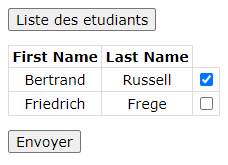
\includegraphics[width=5cm]{assets/attendance.PNG}
            \caption{Page HTML généré par \texttt{RecordAttendance}}
            \label{attendance}        
        \end{center}
    \end{minipage}
\end{figure}

\section{JeSuisEnCours}

Après quelques semaines, nous nous sommes rendus compte que la direction du projet était incompatible avec les exigences administratives. En effet, l'application prévoyait un simple appel du professeur, or l'étudiant doit personnellement attester de sa présence en émargeant un document. Il donc été décidé d'abandonner le projet intiale Attendance pour se tourner vers une application JeSuisEnCours, spécialisée dans la digitalisation les feuilles de présences. 

Le but principal du projet est donc devenu la connexion de l'application JeSuisEnCours aux données de l'université, d'une part, pour accéder aux données (annuaires, emploies du temps,...), d'autre part pour gérer les éléments renvoyés par l'application (absence, justificatif,...).

Malheureursement, la crise sanitaire a fortement ralentit les contacts avec l'équipe de JeSuisEnCours et le projet a finalement été abandonné.
 
\chapter[Plaquette-MIDO]{Plaquette-MIDO\raisebox{.3\baselineskip}{\normalsize\footnotemark}}
\footnotetext{\url{https://github.com/Dauphine-MIDO/plaquette-MIDO}}

Ce projet a pour but d'implémenter un code générant un fichier PDF détaillant les différents enseignements du Master 1 MIAGE en apprentissage à partir de la base de données de Dauphine. La finalité est d'automatiser le lancement du code du sorte que quotidiennement le fichier PDF soit mis à jour et publié en ligne.

À mon arrivée, un code permettait déjà la génération du fichier PDF. Certains passages du code était cependant à revoir pour améliorer l'esthétique du fichier PDF. De plus, le code initial était très peu généralisé à d'autres utilisateurs et plusieurs changements dans le code était nécessaire pour qu'un autre utilisateur puisse lancer Plaquette-MIDO. Il fallait donc davantage généraliser le code de façon à rendre accessible le code à d'autres utilisateurs. Le principal aspect à généraliser était l'authentification à l'API de Dauphine, indispensable pour avoir accès aux données de l'université.

\section{L'authentification}

Pour se connecter à l'API de Dauphine, un nom d'utilisateur et un mot de passe sont nécessaires. Le code initial prévoyait trois manières différentes de fournir ces informations afin de se connecter à l'API :
\begin{itemize}
    \item les propriétés du système
    \item les variables d'environnement
    \item un fichier texte contenant les informations nécessaires
\end{itemize}

Seulement, ce code ne lisait initialement que le mot de passe et le nom d'utilisateur était une valeur par défaut. Un nouvel utilisateur devait donc modifier le code pour pouvoir utiliser ses identifiants. L'idée d'une valeur par défaut pour le nom d'utilisateur a donc abandonné pour rendre le programme plus accessible. La valeur du nom d'utilisateur serait lue de la même manière que celle du mot de passe.

\subsection{La classe Authentication}

Une nouvelle classe a donc été créée pour permettre la généralisation lecture du code et améliorer sa lisibilité. Celle-ci permet de créer un objet contenant un nom d'utilisateur et un mot de passe de type Optional. Ce type permet d'instancer aussi bien la valeur d'une chaîne de caractère que l'absence d'une information. Il permet ainsi de 

\subsection{Le projet CredsRead}
La généralisation du code permettant l'authentification nous a poussé à le séparer dans un projet bien distinct de Plaquette-MIDO, le projet CredsRead. Celui-ci sera ensuite intégré au code source de Plaquette-MIDO.

\section{L'automatisation du lancement du code}

La finalité du projet Plaquette-MIDO est de lancer la construction du fichier PDF quotidiennement et de le publier de manière à ce qu'il soit accessible sur le site de Dauphine. Pour réaliser cette automatisation, j'ai utilisé l'outil Travis-CI.

\subsection{Travis-CI}
    Travis-CI est logiciel d'intégration continue qui permet de compiler,
    tester et déployer le code de dépôts GitHub. Il est configurer à partir
    d'un fichier nommé \texttt{.travis.yml} présent dans la racine du
    répertoire. Celui-ci est lu à chaque nouveau commit par Travis-CI qui
    exécute son contenu sur une machine virtuelle. L'exécution peut alors
    réussir dans le cas où aucune erreur n'a été signalée ou échouer si une
    erreur est survenue. Travis-CI peut donc s'assurer de la bonne
    compilation d'un projet. Il peut également effectuer des déploiements.
    En effet, il est possible d'insérer du script que Travis-CI exécute pour
    déployer des fichiers. Par exemple, ajouter un script avec les commandes
    git adéquat pour pousser des fichiers vers un dépôt. Travis-CI peut donc
    exécuter le code source permettant la création du fichier PDF et ensuite
    déployer ce fichier vers un dépôt GitHub.

\begin{figure}[!h]
    \begin{center}
    %taille de l'image en largeur
    %remplacer "width" par "height" pour régler la hauteur
    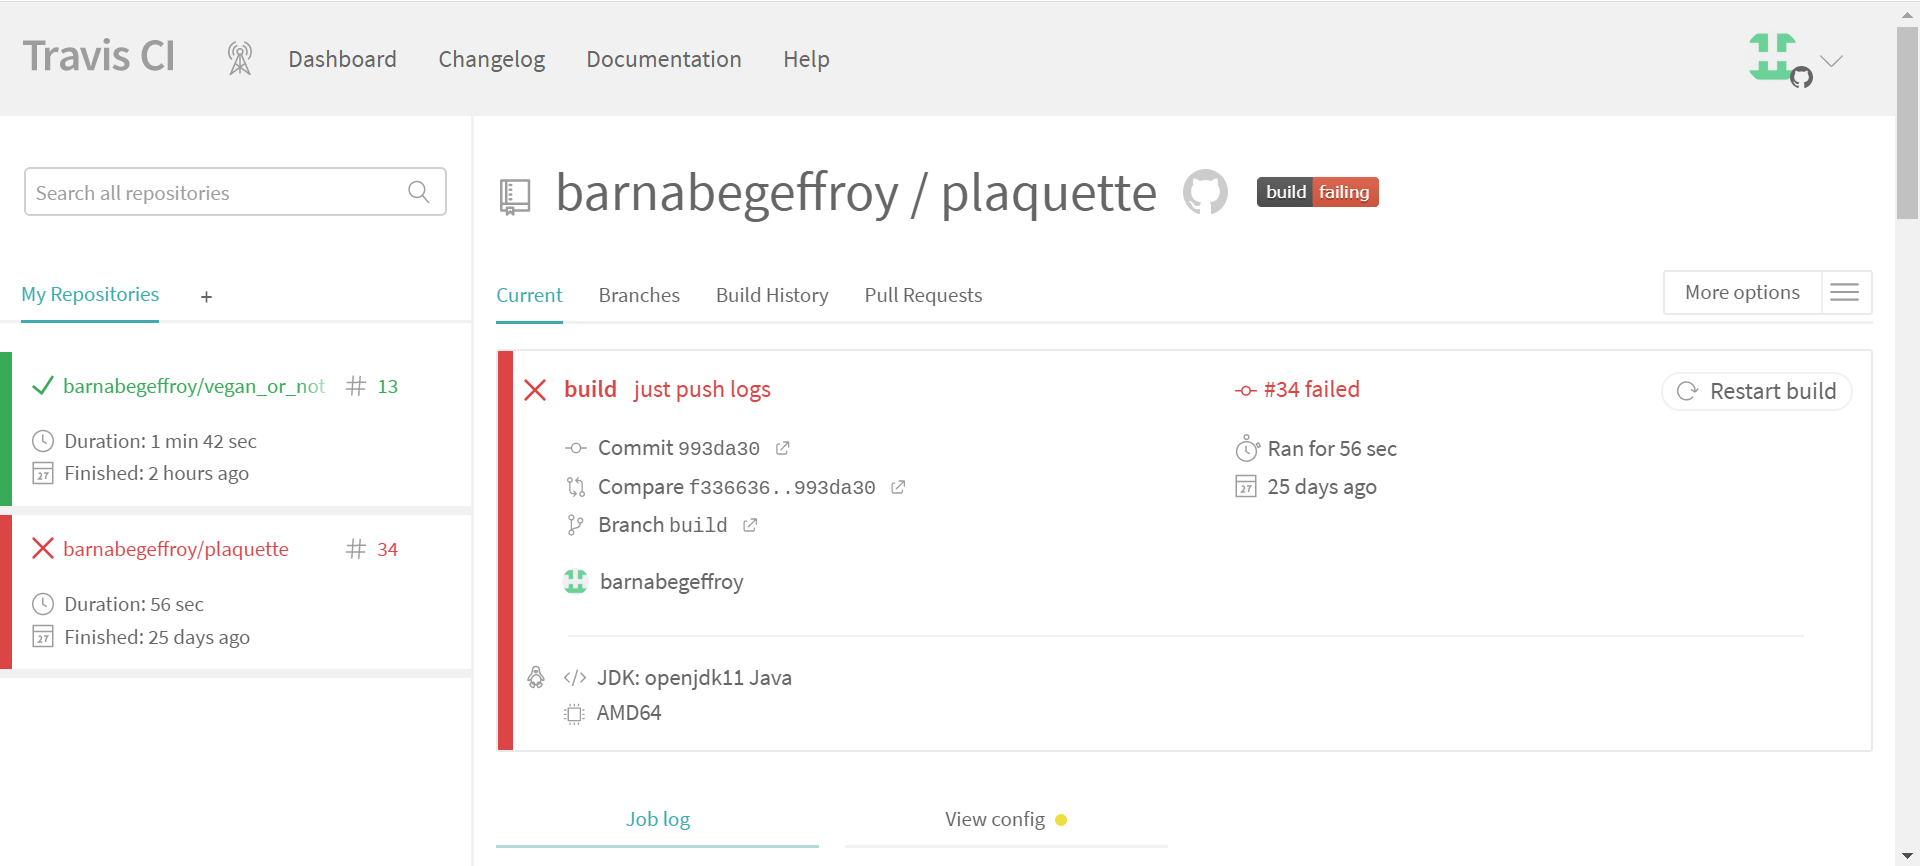
\includegraphics[width=13cm]{assets/travis-ci.PNG}
    \end{center}
    %légende de l'image
    \caption{Enveloppe d'un son}
\end{figure}


Travis-CI permet également de référencer des variables d'environnement sécurisées (clefs d'accès, identifiants,...)
\begin{figure}[!h]
    \begin{center}
    %taille de l'image en largeur
    %remplacer "width" par "height" pour régler la hauteur
    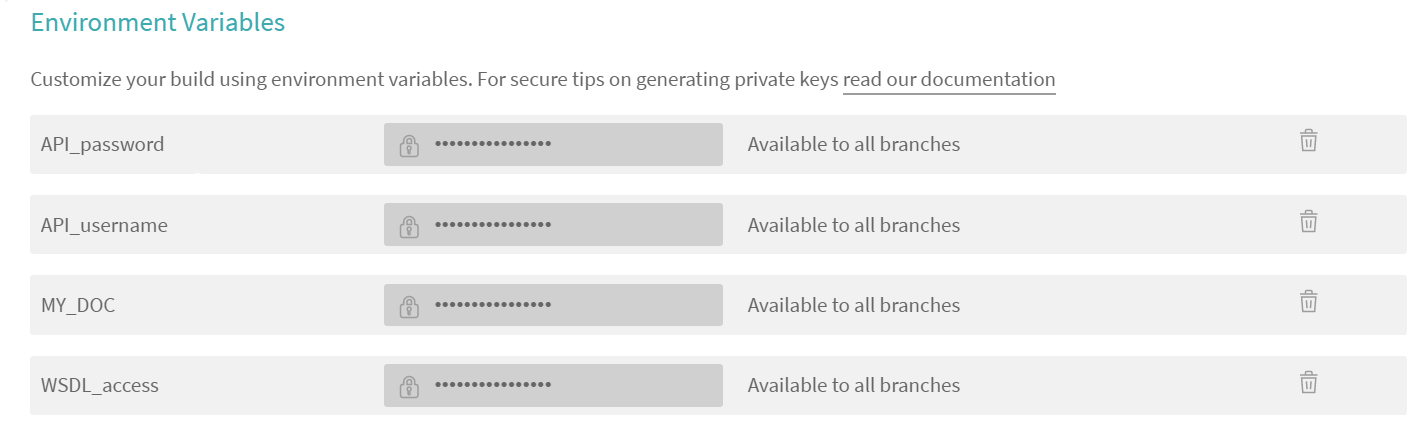
\includegraphics[width=13cm]{assets/env.PNG}
    \end{center}
    %légende de l'image
    \caption{Enveloppe d'un son}
\end{figure}

\subsection{L'exécution du code}
\subsubsection*{Les dépendances}



Travis-CI identifie automatiquement un projet Maven et installe les dépendances indiquées dans le \texttt{pom.xml}. Dans le projet Plaquette-MIDO, la dépendance qui importe le code source de l'API de Dauphine nécessite un fichier texte nommé \texttt{WSDL\_Login.txt} contenant un URL spécifique des identifiants de l'utilisateur. Ce fichier ne peut pas être dans le dépôt car il contient des informations personnelles. Il faut donc un script qui crée le fichier sur la machine virtuelle de Travis-CI. Avant de lancer l'installation des dépendances le fichier doit donc être créer. Dans le \texttt{.travis.yml}, on peut ajouter un script qui génère ce fichier.

\subsubsection*{Création du fichier PDF et déploiement}
Une fois que toutes les dépendances du projet Maven sont installées, il faut executé le code source qui génère le fichier PDF. La méthode main a executé se trouve dans la classe \texttt{M1ApprBuilder.java}. Le déploiement vers le dépôt d'arrivée doit également être pris en compte. Voici le script exécuté par Travis-CI pour réaliser ce travail :


\subsubsection*{Automatisation}
Travis-CI lance initiallement la construction du code à chaque nouveau commit. Il est cependant possible de configurer des \textit{Cron Jobs}. Ceux-ci vont renouveler la construction du code de manière quotidienne, hebdomadaire ou mensuelle. 

\begin{figure}[!h]
    \begin{center}
    %taille de l'image en largeur
    %remplacer "width" par "height" pour régler la hauteur
    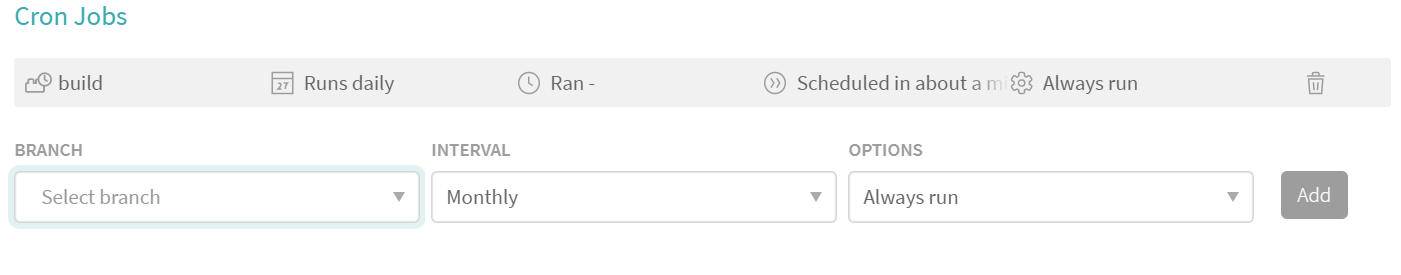
\includegraphics[width=13cm]{assets/CronJobs.PNG}
    \end{center}
    %légende de l'image
    \caption{Enveloppe d'un son}
\end{figure}

En programmant sur \textit{Daily}, Travis-CI va relancer la construction du code tous les jours et ainsi renouveller le fichier PDF et les logs si des changements sont effectués. Si une erreur se produit et que le fichier PDF n'est pas généré, une e-mail nous previendra de la non-construction du code et le fichier PDF le plus récent sera toujours disponible sur le site.

\chapter[CredsRead]{CredsRead\raisebox{.3\baselineskip}{\normalsize\footnotemark}}
\footnotetext{\url{https://github.com/oliviercailloux/creds-read}}

CredsRead, pour Credentials Read, gère comme son nom l'indique la lecture des identifiants d'un utilisateur. Celle-ci s'effectue à trois manières, comme pour l'authenfication dans Plaquette-MIDO, les propriétés du système, les variables d'environnement et un fichier texte.

\section{Diagramme de classe}
Le diagramme de classe permet de avoir une idée précise du code que l'on veut écrire. Papyrus est un outil permettant de réaliser ce genre de diagramme. Son interface intuitive facilite la rédaction d'un diagramme UML(le langage standard des diagrammes de classe) lisible et rigoureux. 

\begin{figure}[!h]
    \begin{center}
    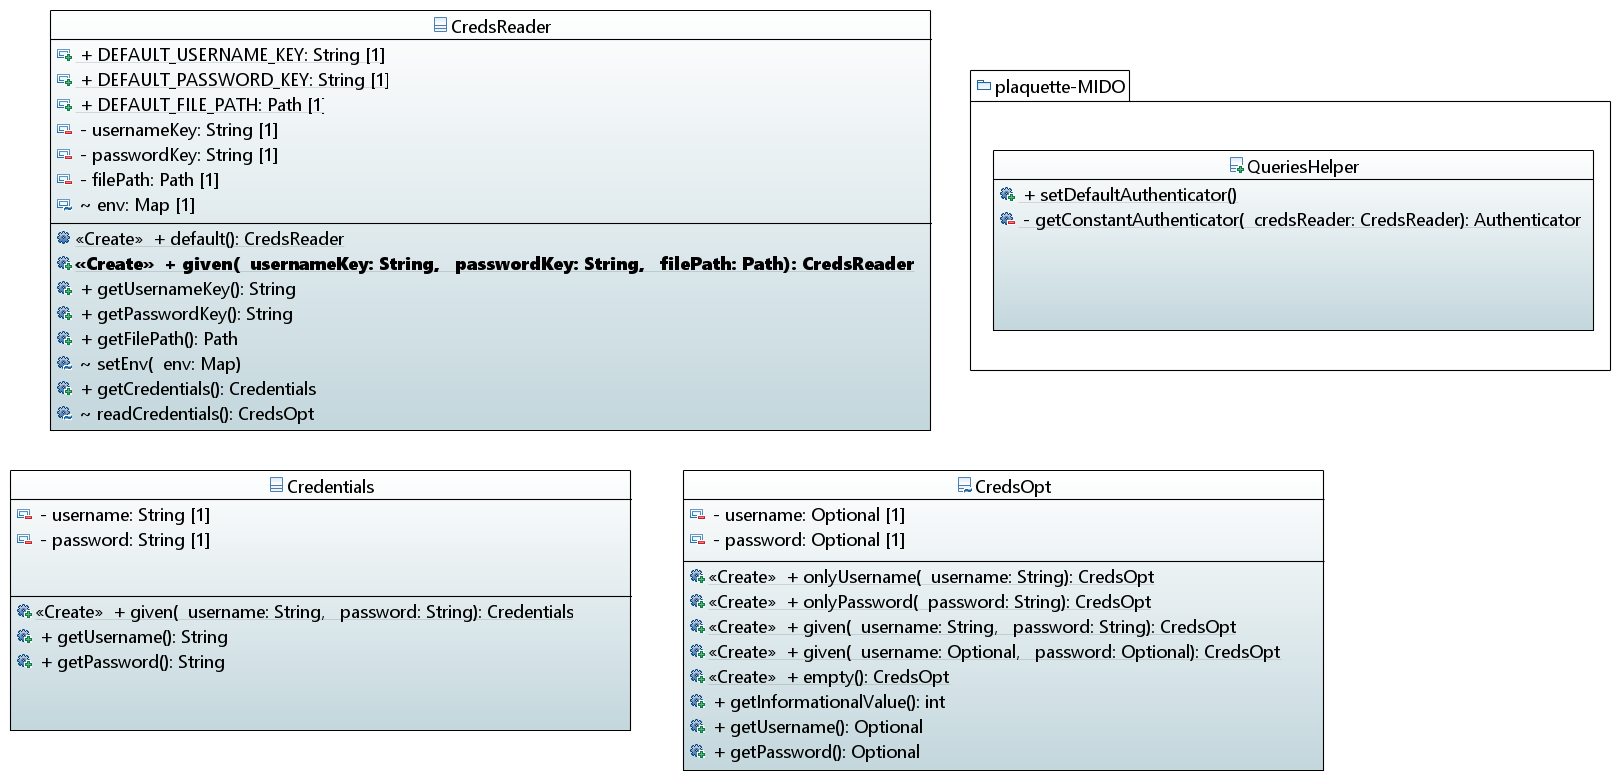
\includegraphics[width=\textwidth]{assets/doc.png}
    \end{center}
    \caption{Diagramme de classe du projet CredsRead}
\end{figure}


Le projet est donc composé de trois classes représentées par les différents blocs. Chaque bloc est composé de son nom, suivi d'une partie avec l'ensemble des variables de la classe, et d'une partie avec l'ensemble des méthodes de la classe. Les éléments soulignés sont des statiques. Le symbole $+$ précédant les éléments indique qu'ils sont publiques, le $-$ privés, le $\sim$ de visibilité package\footnote{En dehors du projet, ces éléments ne sont pas accessibles.}. Les méthodes sont présentés de cette façon \texttt{nomDeMethode(paramètres d'entrée): objet de sortie}. Le préfixe \texttt{Create} indique que ce sont des méthodes de construction. Il y a également un sous-dossier de plaquette-MIDO contenant la classe \texttt{QueriesHelper}. Celle-ci ne contient plus que deux méthodes spécifiques à la connexion à l'API de Dauphine.


\section{Les différentes classes}

\subsection{\texttt{CredsOpt}}
Cette classe remplace la classe \texttt{Authentication}, elle crée un objet contenant les identifiants de l'utlisateur, le nom d'utilisateur et le mot de passe, avec le type \texttt{Optional}. Celle-ci permet d'instancer également l'abscence d'information avec un \texttt{Optional} vide. Une distinction est donc faite entre un \texttt{Optional} vide (absence d'information) et un \texttt{String} vide : \texttt{""}. Ce dernier représente un nom d'utilisateur ou un mot de passe vide. La méthode \texttt{getInformationValue()} renvoie le nombre d'informations présentes (différente d'un \texttt{Optional} vide) dans l'objet \texttt{CredsOpt} (0, 1 ou 2).

Cette classe est de visibilité package, elle n'est utilisée que par les autres classes du package et n'est pas accessible publiquement.

\subsection{\texttt{Credentials}}
Cette classe crée également un objet contenant les identifiants, le nom d'utilisateur et le mot de passe. Ceux-ci sont cette fois de type \texttt{String}. Par rapport à \texttt{CredsOpt}, cette classe, ne permet pas d'instancer l'abscence d'information. 

Cette classe est publique, elle peut donc être utilisée en dehors du package par les utilisateurs.

\subsection{\texttt{CredsReader}}
\texttt{CredsReader} est la classe principale du projet. Elle est instancée par trois variables : une clé pour le nom d'utilisateur \texttt{usernameKey}, une clé pour le mot de passe \texttt{passwordKey} et un chemin vers un fichier \texttt{filePath}. Les deux clés sont utilisées pour lire les propriétés du système et les variables d'environnement. Le chemin correspond au fichier texte contenant les informations d'identification.

L'utilisateur peut créer un objet \texttt{CredsReader} en utilisant ses propres noms pour les variables d'instances. Il peut aussi utiliser les valeurs par défaut de la classe : \texttt{API\_username}, \texttt{API\_password}, \texttt{API\_login.txt}. Ces derniers sont ceux utlisés dans plaquette-MIDO.

\subsubsection{\texttt{readCredentials()}}
Voir annexe~\ref{sec:readCredentials()}.

\texttt{readCredentials()} est la méthode la plus importante de la classe. Elle est de visibilité package, donc elle n'est pas accessible aux utilisateur. Elle renvoie un \texttt{CredsOpt}.

Elle permet de lire les informations d'identification : nom d'utilisateur et mot de passe. Pour chaque information, on distingue l'information manquante et la \texttt{String} vide. La méthode prend en compte les sources possibles suivantes :

\begin{enumerate}
    \item l.3 à 11 : Propriétés du système. Chaque propriété peut être définie, y compris pour la chaîne vide, ou non définie. Une information est considérée comme manquante (dans la source des propriétés) si la propriété correspondante n'est pas définie.
    \item l.13 à 21 : Variables d'environnement. Chaque variable peut être définie, y compris par une chaîne vide, ou non définie. Une information est considérée comme manquante (dans la source des variables d'environnement) si la variable d'environnement correspondante n'est pas définie.
    \item l.23 à 55: Fichier texte. Les deux informations sont considérées comme manquantes (de la source des fichiers) si le fichier n'existe pas. Si le fichier existe, aucune information n'est considérée comme manquante. La première ligne du fichier donne le nom d'utilisateur, la seconde le mot de passe. Si le fichier n'a qu'une seule ligne, le mot de passe (provenant de la source des fichiers) est mis à vide. Si le fichier est vide, les deux informations (provenant de la source des fichiers) sont fixées à la \texttt{String} vide. Les lignes vides ne sont pas prises en compte du tout. Si le fichier ne contient pas de ligne vide après la deuxième ligne, une exception est lancée.
\end{enumerate}
l.51 à 61 : La méthode a une logique de meilleure information de connexion. La source utilisée pour renvoyer un \texttt{CredsOpt} contenant les informations est celle qui a la valeur informationnelle la plus élevée, telle que déterminée par \texttt{CredsOpt.getInformationalValue()} (ce qui signifie que les sources sont classées par ordre croissant du nombre d'informations manquantes), et, dans le cas d'un fichier ex-\ae quo, l'ordre de priorité, tel que présenté ci-dessus, détermine quelle source est choisie.

\subsubsection{\texttt{getCredentials()}}
Voir annexe~\ref{sec:getCredentials()}

\texttt{getCredentials()} est la classe publique renvoyant un \texttt{Credentials}. Elle utlise la méthode \texttt{readCredentials()} pour récupérer la meilleure information d'identification (logique de priorité). Elle lance une exception si une (ou les deux) information manque.

\section{Intégration à plaquette-MIDO}

Le projet CredsRead a d'abord été édité dans le projet Plaquette-MIDO. Il a ensuite été séparé du projet initial. Il fallait donc l'intégrer. Pour cela, le projet CredsRead est publié sur Maven Central. Le projet peut donc être intégré à plaquette-MIDO en l'ajoutant dans le \texttt{pom.xml} et de cette façon l'utiliser dans la classe \texttt{QueriesHelper} de plaquette-MIDO.

\begin{figure}[!ht]
    \lstinputlisting[language=Java, firstline=9, lastline=28]{assets/QueriesHelper.java}
    \caption*{La classe \texttt{QueriesHelper}, utilisant le projet CredsRead pour plaquette-MIDO.}
\end{figure}

\chapter[Jugement délibéré, les régimes alimentaires]{Jugement délibéré, les régimes alimentaires\raisebox{.3\baselineskip}{\normalsize\footnotemark}}
\footnotetext{\url{https://github.com/barnabegeffroy/vegan_or_not}}
Ce projet a pour but de mettre en pratique les théories exposées dans l'article \textit{A formal framework for deliberated judgment}\cite{cailloux_formal_2020}. Cette article de théorie du choix s'intéresse à l'influence des arguments dans la prise de décision. Le jugement délibéré est le fait de prendre une décision en ayant pris en compte différents arguments qui ne vous feront pas changer d'avis. Pour avoir des données empiriques sur ce modèle, il a été convenu de s'intéresser aux régimes alimentaires proposés dans une cantine.

\section{Protocole de l'expérience}
L'idée est de proposer aux utilisateurs un site web sur lequel l'influence des arguments dans leur assentiment à une cantine végane ou non est suivie. Pour cela le site web proposera des vidéos de deux experts, un en faveur des régimes véganes, l'autre contre ce genre de régimes alimentaires. L'utilisateur aura accès à une bibliothèque de vidéos d'arguments des deux experts. Cette bibliothèque sera dynamique et évoluera en fonction des vidéos vues. Si l'utilisateur a vu l'argument 1 de l'expert A, il aura alors accès à la réponse de l'expert B, le contre-argument. Si ensuite, il visionne ce contre-argument, il aura accès au contre-contre-argument de l'expert A, et ainsi de suite jusqu'à ce que le débat sur cet argument soit clos par l'un des experts. Le site web doit également proposer des formulaires, en fonction des vidéos visionnées, afin de capturer la tendance de l'opinion de l'utilisateur et le moment où celui-ci émettra un jugement délibéré. Ces formulaires permettront d'étudier la puissance des arguments des deux experts et la tendance des utilisateurs dans leur prise de décision. Outre ces formulaires, le site web doit fournir des informations techniques sur le parcours de l'utilisateur, notamment le temps de visionnage des différentes vidéos.

\section{Création d'un site web}
Le site web doit répondre aux exigences du protocole : 
\begin{itemize}
    \item proposer une bibliothèque de vidéos dynamique.
    \item fournir des formulaires adaptés aux vidéos visionnées.
    \item récupérer les données de l'utilisateur sur le visionnage des vidéos.
\end{itemize}
En ce qui concerne le premier et dernier point, ils sont fortement liés. En effet, une fonction pourrait permettre de débloquer la réponse à un argument une fois que l'information "vidéo lue jusqu'à la fin" serait transmise. Pour réaliser cela, \textit{video.js}, lecteur open source, permet d'obtenir de nombreuses données nécessaires pour le projet.

Ce projet a été réalisé avec une étudiante en nutrition, il fallait alors également trouver une interface opensource permettant d'éditer un site web facilement.

\subsection{WordPress}
WordPress est un logiciel de conception web (CMS). Il est utilisé par 35\% des sites web dans le monde. WordPress permet de réaliser un site web de qualité sans avoir besoin de compétences techniques importantes (HTML, JavaScript). Il propose différents modèles adaptables facilement et plus de 30 000 extensions permettant d'accéder facilement à de multiples fonctionnalités (vidéos, formulaires, analyse de fréquentations, ...). WordPress semble ainsi être l'interface opensource parfaite pour éditer le site web facilement tout en respectant le protocole.

\begin{figure}[!ht]
    \begin{center}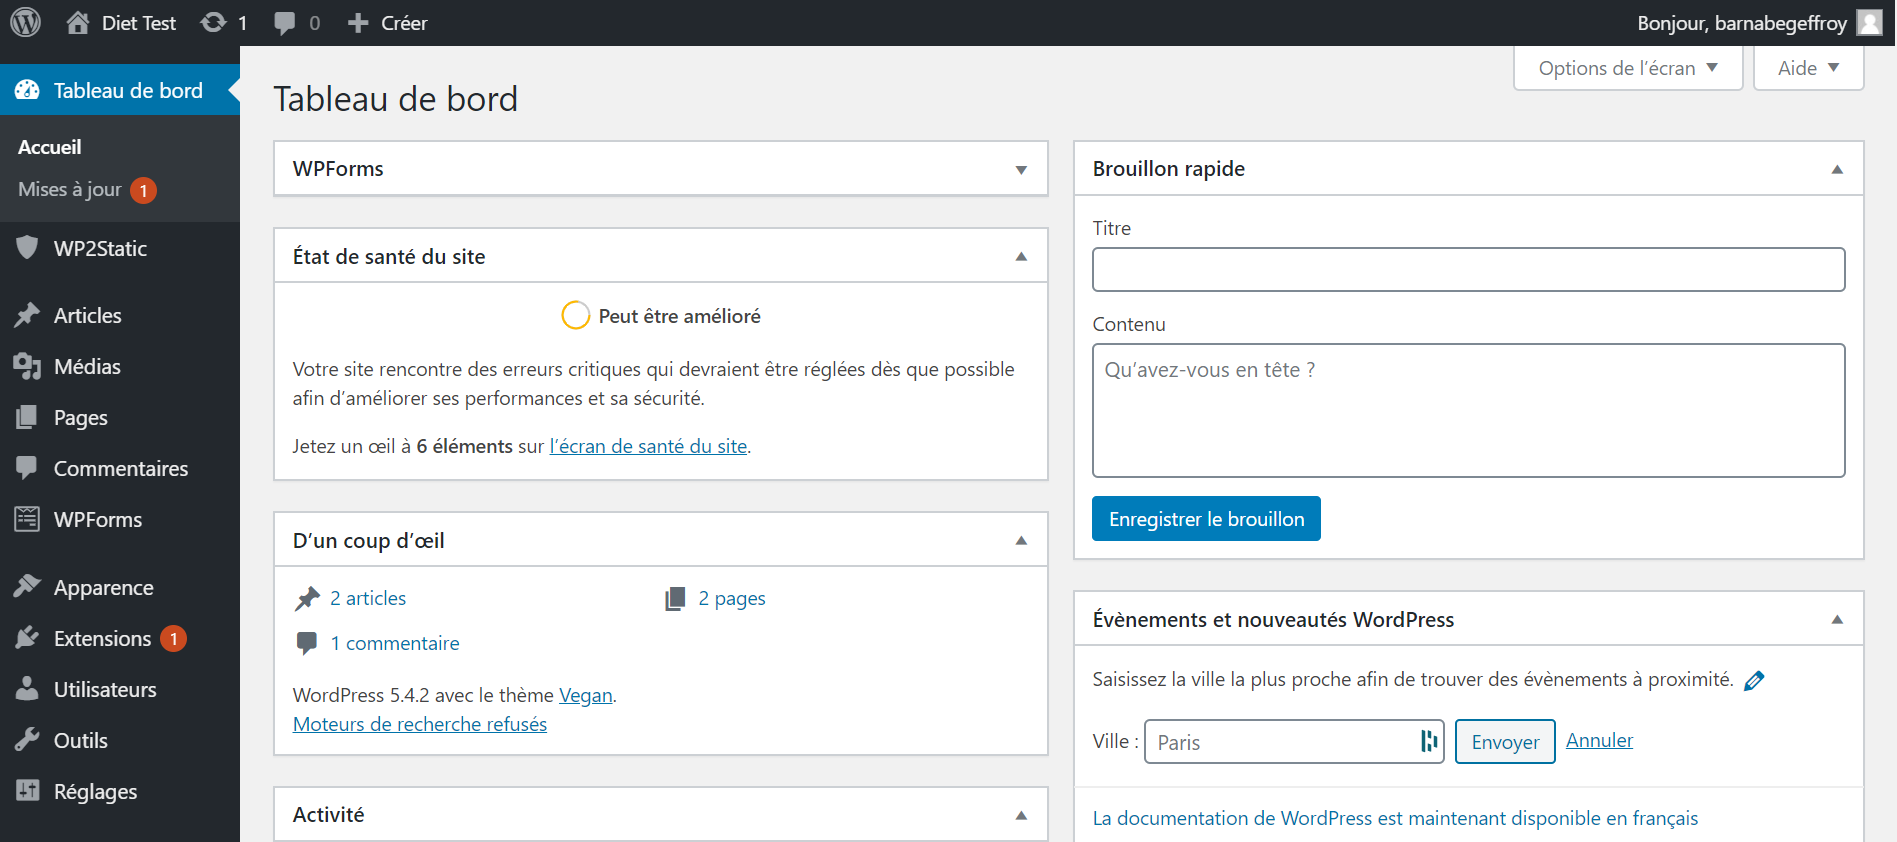
\includegraphics[width=\textwidth]{assets/wp.PNG}
    \end{center}
    \caption{Capture d'écran de l'interface de WordPress}
\end{figure}
Une contrainte s'ajoutait tout de même en utilisant WordPress. Le fait de dépendre d'extensions pouvant évoluer et ne plus être compatible avec nos exigeances était en effet un risque à éviter. De plus, le code source est très peu accessible sur WordPress, il est très compliqué de réaliser un site web sur mesure lorsque celui-ci exige des points techniques très précis.

Il a donc été décidé de concevoir l'esthétique du site sur WordPress (affichage, thème, polices, images). La partie technique (dynamisme, récupération des données) serait développée sur Jekyll.

\subsection{Jekyll}
\subsubsection{Fonctionnement}
Jekyll est un générateur de site statique\footnote{Une page web statique est une page web dont le contenu ne varie pas en fonction des caractéristiques de la demande.}. Ce logiciel permet de générer facilement une architecture web convaincante. Jekyll propose un système de modèle de page. Celui-ci permet d'obtenir des pages suivant les mêmes caractéristiques (styles, en-tête, pied de page, barre de navigation, ...) sans recopier sur chaque page le code HTML nécessaire. Le code permet également la conversion de fichier Markdown\footnote{Markdown est un langage de balisage offrant une syntaxe facile à lire et à écrire.}, éditable facilement, en page HTML. Chaque fichier doit er par une en-tête lue par Jekyll (voir ci-dessous). Celle-ci contient les informations permettant à Jekyll de générer une page HTML. Le fichier ne peut contenir que cette en-tête, comme ci-dessous.
\begin{figure}[!ht]
\begin{lstlisting}[language=Ruby]
---
layout: post
title:  "Le premier argmuent de l'expert A!"
date:   2020-03-27
excerpt: "S1a"
image : {{page.image}}
---
\end{lstlisting}
\caption*{Contenu d'un fichier suivant le modèle \texttt{post} pour générer une page vidéo}
\end{figure}

Jekyll va, en suivant ces quelques lignes suivrent, générer la page web (voir figure~\ref{s1a}) à partir du modèles post. L'annexe~\ref{sec:shtml} détaille le code HTML généré par Jekyll et permet de se rendre compte de l'efficacité de Jekyll, seulement sept lignes de code ont suffit à générer 190 lignes de code HTML. La page contient une vidéo qui est généré par l'\texttt{excerpt} (l.72 à 75).

\vspace{1cm}
\begin{figure}[!ht]
    \begin{center}
        
\includegraphics[width=0.8\textwidth]{assets/s1a.PNG}
        \caption{Capture d'écran de la page web généré par les lignes de codes ci-dessus}
        \label{s1a}
    \end{center}
\end{figure}

\subsubsection{Thèmes}
Jekyll possède une bibliothèque de thème opensource avec des nombreux modèles préexistants. Le thème de la figure~\ref{s1a} avait d'abord été choisi en attendant de récuprer les données esthétiques du site WordPress. Cependant ce thème présentait quelques disfonctionnements et le thème de la figure a finalement été choisi

\begin{figure}[!h]
    \begin{center}
    
\includegraphics[width=0.7\textwidth]{assets/newtheme.PNG}
    \end{center}
    \caption{Nouveau thème Jekyll utilisé provisoirement dans l'attente de l'esthétique WordPress}
\end{figure}

\section{Déploiement sur Internet}
\subsection{Jekyll}
Jekyll a été créé par le fondateur de GitHub, Tom Preston-Werner. Son déploiement sur Jekyll est relativement simple. Il suffit de déposer les fichiers générés par Jekyll sur un dépôt GitHub pour que ceux-ci soient déployés sur un site web, une page GitHub.

La génération des fichiers par Jekyll est automatisé de la même manière que plaquette-MIDO avec Travis-CI (voir section~\ref{sec:automatisation}). Le dépôt vers lequel les fichiers sont déployés est \href{https://github.com/barnabegeffroy/vegan_or_not}{\textcolor{blue}{\underline{vegan\_or\_not}}}. GitHub va donc créer une page GitHub à partir du contenu de ce dépôt. On obtient ainsi notre site web, \href{https://barnabegeffroy.github.io/vegan_or_not/}{\textcolor{blue}{\underline{Vegan or not vegan}}}.

\subsection{WordPress}
Le déploiement de la page WordPress sur Internet est un peu plus complexe. Pour un déploiement optimal, WordPress préconise de passer par un hébergeur web adapté et payant. Une extension WordPress existe cepandant pour convertir le contenu WordPress en statique, lisible par GitHub pour générer une page GitHub. Cette extension s'appelle WP2Static. Elle crée un répertoire contenant les fichiers statiques. Il suffit de pousser ces derniers vers un dépôt GitHub pour que le site web soit déployé. Un exemple de page WordPress déployé sur une page GitHub est disponible sur ce \href{https://barnabegeffroy.github.io/static-wp/}{\textcolor{blue}{\underline{lien}}}.

\chapter*{Remerciements}

\addcontentsline{toc}{chapter}{Remerciements}
Je remercie chaudement Olivier Cailloux qui m’a suivi tout au long de ce stage. Premièrement, il a accepté de m'encadrer malgré mon peu d'expérience en développement. Secondement, très pédagogue et à l’écoute, il a su me transmettre son goût pour l'informatique. Le partage de ses cours m'a été d'une grande aide à la compréhension des travaux à réaliser. Je le remercie également pour sa patience dans la relecture de mes codes parfois archaïques et pour nos périodes de riches échanges. Je garderai un très bon souvenir de cette période pratique.

\vspace{30pt}
{\let\clearpage\relax\chapter*{Conclusion
}}
\addcontentsline{toc}{chapter}{Conclusion}

Ce stage m'aura ainsi permis de découvrir davantage le domaine du développement informatique. À travers les différents projets menés, j'ai pu explorer différentes voies du développement : site web, projets Maven/Java, intégration continue... et de maîtriser de nombreux outils et langages informatiques : \texttt{Git}, Travis-CI, Jekyll, Maven, WordPress, HTML, JavaScript... Ce stage m’a ainsi fortement conforté dans le choix d'une formation axée sur l'informatique et le développement.



\newpage
\pagenumbering{roman}
%Ne pas numéroter cette partie

\part*{Annexes}
\addcontentsline{toc}{part}{Annexes}
\newpage
%Rajouter la ligne "Annexes" dans le sommaire

\chapter*{Annexe 1}
\addcontentsline{toc}{chapter}{Annexe 1}

%changer le format des sections, subsections pour apparaittre sans le num de chapitre
\makeatletter
\renewcommand{\thesection}{\@arabic\c@section}
\makeatother

%recommencer la numérotation des section à "1"
\setcounter{section}{0}

Intro

\section{Partie 1}

Bla

\subsection*{writeWSDL.sh}
\lstinputlisting[language=bash, firstline=18]{./assets/writeWSDL.sh}

\subsection*{cibuild.sh}
\lstinputlisting[language=bash]{./assets/cibuild.sh}

\chapter*{Codes CredsRead}
\addcontentsline{toc}{chapter}{Codes CredsRead}

%changer le format des sections, subsections pour apparaittre sans le num de chapitre
\makeatletter
\renewcommand{\thesection}{\@arabic\c@section}
\makeatother

%recommencer la numérotation des section à "1"


\section{Classe CredsReader}

\subsection{Méthode readCredentials()}
\label{sec:readCredentials()}
\lstinputlisting[language=Java, firstline=166, lastline=227]{./assets/CredsRead.java}

\vspace{1cm}

\subsection{Méthode getCredentials()}
\label{sec:getCredentials()}
\lstinputlisting[language=Java, firstline=133, lastline=152]{./assets/CredsRead.java}

\newpage

%récupérer les citation avec "/footnotemark"
\nocite{*}

%choix du style de la biblio
\bibliographystyle{plain}
%inclusion de la biblio
\bibliography{bibliographie.bib}
%voir wiki pour plus d'information sur la syntaxe des entrées d'une bibliographie
\thispagestyle{empty}
\setcounter{page}{0}

\end{document}